\newpage
\title{LEZIONE 7 19/03/2020}\newline
\textbf{link} \href{https://web.microsoftstream.com/video/2feefb06-11cb-4de4-ac19-dcc5fe175a98?list=user&userId=faa91214-a6f5-40d7-8875-253fd49b8ce1}{clicca qui}
\section{Esercizi di ricapitolazione degli argomenti fino ad ora trattati}
\subsection{Es. Equilibri e stabilità in un sistema non lineare, TDE 06/05/2014 E1} Dato il SD NL a TC:
\[
    \begin{cases}
        \dot{x_1} = x_1^3 + x_2 + u\\
        \dot{x_2} = x_1 e^{x_2}\\
        y = x_1 (x_2 - u) + u^2
    \end{cases}
\]
Domande:
\begin{itemize}
    \item Trovare gli stati e le uscite di equilibrio per $u(t) = \bar{u} = -1$;
    \item Trovare le stabilità degli equilibri eventualmente trovati al punto precedente.
\end{itemize}
\ \newline
\textbf{Equilibri}:\newline
essendo a TC, la caratteristica degli equilibri è che le derivate dello stato sono nulle (devono essere ferme)
\[
    \bar{x}_1^3 + \bar{x}_2 + \bar{u} = 0
\]
\[
    \bar{x}_1 e^{\bar{x}_2} = 0
\]
Con la seconda equazione ricaviamo immediatamente che $\bar{x}_1 = 0$ e con la prima equazione invece ricaviamo che $\bar{x}_2 = - \bar{u}$.\newline
Quindi per $\bar{u} = -1$ esiste il solo equilibrio 
$\bar{x} = \left[\begin{matrix}
    0 \\ 
    1
\end{matrix}\right]$.\newline
Stato dell'uscita d'equilibrio:
\[
    \bar{y} = \bar{x} (\bar{x}_2 - \bar{u}) + \bar{u}^2 = 1
\]
\newline
\textbf{Sistema linearizzato e stabilità degli equilibri}:\newline
Ripasso dei criteri:
\begin{itemize}
    \item Sistema linearizzato è asintoticamente stabile, ($\Rightarrow$) allora abbiamo un equilibrio asintoticamente stabile.
    \item Matrice $A$ del sistema linearizzato con almento un autovalore con parte reale positiva, ($\Rightarrow $) allora equilibrio instabile.\newline
    \textbf{oss.} un sistema lineare (o linearizzato) può essere instabile anche senza avere autovalore con parte positiva (ricontrolla la teoria per saperne di più).
    \item Altrimenti non si può dire nulla, può essere qualunque cosa.
\end{itemize}
Applichiamo questi criteri:\newline
Calcoliamo $f_x = \left[\begin{matrix}
    3x_1^2 & 1 \\
    e^{x_2} & x_1 e^{x_2}
\end{matrix}\right]$. \newline
Nell'equilibrio $f_x |_{\bar{x}, \bar{u}}=  [\bar{x}_1 = 0, \bar{x}_2 = 1, \bar{u} = -1] = \left[\begin{matrix}
    0 & 1 \\ e & 0
\end{matrix}\right]$.\newline
Autovalori: $\;\;\;\;\;det \left[\begin{matrix}
    s & -1 \\ -e & s
\end{matrix}\right] = 0 \;\;\;\;\; \rightarrow  \;\;\;\;\; s^2 - e = 0 \;\;\;\;\;$, quindi abbiamo un autovalore con parte reale positiva e quindi siamo in presenza di un equilibrio instabile.\newline
\rule{\textwidth}{0,4pt}
\subsection{Es. Stabilità, funzione di trasferimento e calcolo del movimento forzato con Heaviside, TDE 04/05/2015 E1}
Dato il SD LTI SISO a TC 
\[
    \begin{cases}
        \dot{x} = \left[\begin{matrix}
            -11 & 9 \\ -12 & 10 
        \end{matrix}\right]x + \left[\begin{matrix}
            -3\\-3
        \end{matrix}\right] u \\
        \\
        y = \left[\begin{matrix}
            2 &1
        \end{matrix}\right] x
    \end{cases}
\]
determinare
\begin{itemize}
    \item Se è asintoticamente stabile, stabile o instabile;
    \item la funzione di trasfermineto $G(s)$;
    \item $y(t)$ prodotto da $x(0) = \left[\begin{matrix}
        0\\0
    \end{matrix}\right]$ (cioè solo movimento forzato) e $u(t) = 2 sca(t)$. 
\end{itemize}
\textbf{Stabilità}:\newline
Autovalori di $A$:
\[
    det \left[\begin{matrix}
        s +11 & -9 \\ 12 & s-10
    \end{matrix}\right] = 0 \;\;\;\;\;\rightarrow \;\;\;\;\; s^2 + s -110 +108 = 0 \;\;\;\;\; \rightarrow  \;\;\;\;\; s^2 + s -2 = 0
\]
Abbiamo una variazione di segno e un autovalore con parte reale positiva, quindi il sistema è instabile.\newline
La risposta a questa domanda termina qua, senza dover calcolare gli autovalori, ma noi proseguiamo coi conti, perchè tanto ci servono per i punti successivi.\newline
\[
    s_{1,2} = - \frac{1}{2} \mp \sqrt{\frac{1}{4} + 2} = - \frac{1}{2} \mp \sqrt{\frac{9}{4}} = \begin{cases}
        -2\\ 1
    \end{cases}
\]
\textbf{Funzione di trasferimento}:
\[
    G(s) = c(sI-A)^{-1} b +d = \left[\begin{matrix}
        2 &1
    \end{matrix}\right] \left[\begin{matrix}
        s+11 & -9 \\ 12 & s-10
    \end{matrix}\right]^{-1} \left[\begin{matrix}
        -3\\-3
    \end{matrix}\right] =
\]
[per il calcolo della inversa di una matrice 2x2 (solo e soltanto 2x2) si moltiplica $\frac{1}{det(matrice)}$ per la matrice ottenuta cambiando di posizione i termini della diagonale principale e invertendo i segni dei termini della diagonale secondaria]
\[
    = \frac{1}{s(+2)(s-1)} \left[\begin{matrix}
        2 &1
    \end{matrix}\right] \left[\begin{matrix}
        s-10 & 9 \\ -12 & s+11
    \end{matrix}\right] \left[\begin{matrix}
        -3\\-3
    \end{matrix}\right] = \frac{1}{s(+2)(s-1)} \left[\begin{matrix}
        2 & 1
    \end{matrix}\right] \left[\begin{matrix}
        -3s+3\\-3s + 3
    \end{matrix}\right] =
\]
\[
    = \frac{1}{s(+2)(s-1)} (-6s + 6 -3s +3) = \frac{-9s +9}{(s+1)(s-1)} = \frac{-9 \cancel{(s-1)}}{(s+2)\cancel{(s-1)}} = \frac{-9}{s+2}
\]
\newline
\textbf{Movimento forzato prodotto da $u(t) = 2 sca(t)$}:\newline
Nella consegna il fatto che si imponga $x(0) = \left[\begin{matrix}
    0\\0
\end{matrix}\right]$ significa che nel calcolo dell'uscita nel dominio delle trasformate, non c'è bisogno di calcolare il movimento libero, perchè è nullo, ma per calcolare l'uscita è sufficiente considerare il movimento forzato:
\[
    U(s) = \frac{2}{s} \;\; \Rightarrow  \;\; Y(s) = G(s) U(s) = - \frac{18}{s(s+2)}
\]
Uso Heaviside:
\[
    U(s) = \frac{\alpha}{s} + \frac{\beta}{s+2}
\]
Denominatore comune e uguaglio i numeratori:
\[
    \alpha(s+2) + \beta s = 18 \;\;\;\; \Rightarrow \;\;\;\; \begin{cases}
        s= 0 \rightarrow \alpha = -9\\
        s = -2 \rightarrow  \beta = 9
    \end{cases}
\]
Quindi 
\[
    Y(s) = -\frac{9}{s} + \frac{9}{s+2}
\]
che antitrasformata mi produce
\[
    y(t) = - 9 sca(t) + 9 e^{-2t} sca(t)) = 9 sca(t) (-1 + e^{-2t})
\]
\rule{\textwidth}{0,4pt}
\subsection{Es Applicazione reale}
Consideriamo un corpo solido riscaldato e che scambia convettivamente temperatura con una temperatura fissa.\newline
[immagine dagli appunti del prof]
\begin{center}
    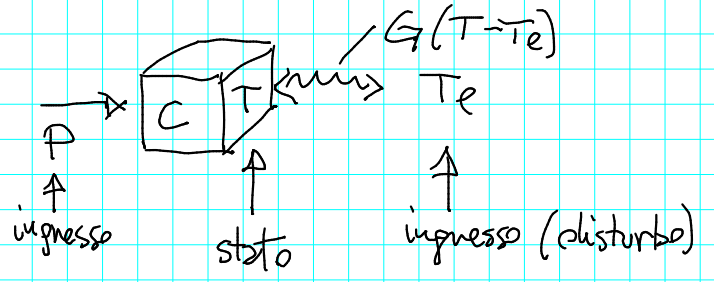
\includegraphics[height=3cm]{../lezione7/img1.PNG}
\end{center}
La potenza termica $P$ e la temperatura fissa $Te$ rappresentano gli ingressi del sistema, la temperatura $T$ del corpo rappresenta lo stato del sistema, inoltre il corpo è caratterizzato da una certa capacità terminca $C$, c'è anche uno scambio termico per convezione con la temperatura fissa e vale $G(T-Te)$, con $G$ una costante chiamata conduttanza termica.\newline
Diciamo che la capacità termica $C=10J/K$, e che la conduttazza termica $G = 2 W/K$
\newline
\newline
\textbf{Modello}:\newline
Bilancio dinamico di energia:
\[
    \frac{d}{dt}E = \sum P
\] con $E = CT$ e $P = P-G(t-Te)$. \newline
Quindi
\[
    C \dot{T} = P - G(T-Te)
\]
\[
    \dot{T} = \frac{1}{C}P - \frac{G}{C} T + \frac{G}{C}Te
\]
\[
    \dot{T} = -\frac{G}{C}T + \frac{1}{C}P + \frac{G}{C}Te
\]
Che è proprio una equazione di stato in cui $\dot{x} = \dot{T}$, $a=-\frac{G}{C}$, $u=\frac{1}{C}P$, distrubo$=\frac{G}{C}Te $.\newline
Trasformiamo secondo Lapalce e guardiamo soltato i movimenti forzati:
\[
    sT(s) = - \frac{G}{C}T(s) + \frac{1}{C}P(s) + \frac{G}{C}Te(s)
\]
\[
    T(s) = \frac{1}{s+ \frac{G}{C}}( \frac{1}{C}P(s) + \frac{G}{C}Te(s)) = \frac{\frac{1}{c}}{s + \frac{G}{C}} P(s) + \frac{\frac{G}{C}}{1 + \frac{G}{C}} Te(s)
\]
Dove il termine $\frac{\frac{1}{c}}{s + \frac{G}{C}} P(s)$ è la funzione di trasferimento da $P$ a $T$, cioè l'effetto di $P$ su $T$, e il termine $\frac{\frac{G}{C}}{1 + \frac{G}{C}} Te(s)$ è la funzione di trasferimento da $Te$ a $T$, cioè l'effetto di $Te$ su $T$.\newline
$T$ è quindi calcolabile con il principio di sovrapposizione degli effetti.\newline
Scriveremo spesso la funzione di trasferimento da un generico $U$ a un generico $Y$ come $\frac{Y(s)}{U(s)}$, ovvero come nel nostro caso:
\[
    T(s) = \frac{T(s)}{P(s)}P(s) + \frac{T(s)}{Te(s)}Te(s)
\]
dove $\frac{T(s)}{p(s)}$ e $\frac{T(s)}{Te(s)}$ sono funzioni di trasferimento e, invece, $P(s)$ e $Te(s)$ sono trasformate di Lapalce degli ingressi/disturbi.\newline
Si può essere tentati dal fatto di fare erroneamente la seguente semplificazione:
\[
    T(s) = \frac{T(s)}{\cancel{P(s)}}\cancel{P(s)} + \frac{T(s)}{\cancel{Te(s)}}\cancel{Te(s)}
\]
L'errore sta nel fatto che i termini $\frac{T(s)}{p(s)}$ e $\frac{T(s)}{Te(s)}$ sono entità uniche, sono funzioni di trasfrimento che vanno lette come $\frac{T_{\text{dovuta a P}}(s)}{p(s)}$ e $\frac{T_{\text{dovuta a Te}}(s)}{Te(s)}$ !\newline
\newline
Riscriviamo le funzioni di trasferimento in modo leggermento diverso:
\[
    \frac{T(s)}{P(s)} = G_{TP}(s)= \frac{\frac{1}{C}}{s + \frac{G}{C}} = \frac{\frac{1}{G}}{1 + \frac{C}{G}s}
\]
\[
    \frac{T(s)}{Te(s)} = G_{TTe}(s) = \frac{\frac{G}{C}}{s+ \frac{G}{C}} = \frac{1}{1 + \frac{C}{G}s}
\]
Supponiamo di applicare uno scalino a $P$, quindi l'ingresso $P(s) = \frac{\bar{P}}{s}$, calcoliamo l'effetto su $T$:
\[
    T(s) = G_{TP}(s) \cdot P(s) = \frac{\frac{1}{G}}{1 + \frac{C}{G}s} \cdot  \frac{\bar{P}}{s} = 
\]
chiamiamo per semplicità $\mu = \frac{1}{G}$ e $\tau = \frac{C}{G}$ 
\[
    T(s) = \frac{\mu}{1 + s \tau} \frac{\bar{P}}{s}
\]
Usiamo ora Heaviside:
\[
    T(s) = \frac{\alpha}{s} + \frac{\beta}{1 + s \tau}
\]
Facendo denominatore comune ed uguagliando i numeratori:
\[
    \alpha(1 + s \tau) + \beta s ) = \mu \bar{P}
\]
Avendo radici $s= 0$ e $ s= - \frac{1}{\tau}$ ottengo:
\[
    \alpha = \mu \bar{P} \;\;\;\;\;\;\;\;\;\;\;\;\;\;\;\beta=-\mu \tau \bar{P}
\]
Quindi:
\[
    T(s) = \frac{\mu \bar{P}}{s} - \frac{\mu \tau \bar{P}}{1 + s \tau} = \frac{\mu \bar{P}}{s} - \frac{\mu \bar{P}}{s + \frac{1}{\tau}}
\]
Antitrasformiamo con le trasformate notevoli:
\[
    \mathcal{L}^{-1}[T(s)] = T(t) = \mu \bar{P} sca(t) - \mu \bar{P} e^{-\frac{t}{\tau}} sca(t) = \mu \bar{P} sca(t) (1- e^{- \frac{t}{\tau}})
\]
[c'è un errore di un $1$ al posto di una $s$ da qualche parte in uno dei passaggi precedenti\dots il prof dice che correggerà i suoi appunti più tardi, quindi per i conti precisi guardare quelli, tanto quel che conta è il ragionamento]\newline
\newline
\textbf{Aspetto della risposta}:\newline
\newline
$T(0) = 0$ (n.b. è l'effetto di $P$, cioè la variazione rispetto all'effetto di $Te$, cioè significa che non si scalda rispetto a $Te$, ma rimane a temperatura di regime $Te$).\newline
\newline
$T(\infty) = \mu \bar{P} = \frac{1}{G}\bar{P}$.\newline
\newline
$\frac{dT}{dt}|_{t=0}$, verifico e calcolo con teorema valore iniziale e teorema valore finale: $T(s) = \frac{\mu \bar{P}}{s(1+s \tau)}$, considerando $\tau> 0$.\newline
1) $T(0^+) = \lim_{s\rightarrow \infty} s T(s) = \lim_{s\rightarrow \infty} \frac{\mu \bar{P}}{1+s \tau} = 0$, verifgicato.\newline
2) $T(\infty) = \lim_{s\rightarrow 0}s T(s) = \lim_{s\rightarrow 0}\frac{\mu \bar{P}}{1 + s\tau} = \mu \bar{P}$, verificato.\newline
$\mathcal{L}[\dot{T}] = s \mathcal{L}[T] - T(0) = \frac{\mu \bar{P}}{1 + s \tau}$\newline
3) $\dot{T}(0) = \lim_{s\rightarrow \infty} s \mathcal{L}[\dot{T}] = \lim_{s\rightarrow \infty}\frac{\mu \bar{P} s}{1+ s \tau} = \frac{\mu \bar{P}}{\tau}$\newline
\newline
Adesso con le equazioni 1), 2) e 3) possiamo disegnare come è fatta:\newline
[immagine dagli appunti del prof]
\begin{center}
    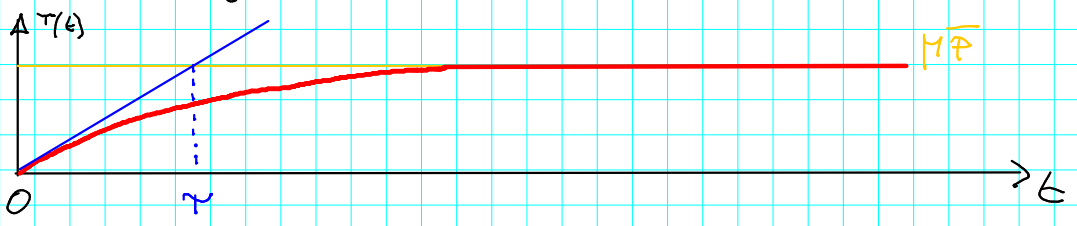
\includegraphics[height=3cm]{../lezione7/img2.PNG}
\end{center}